%!TeX jobName=challenges/stego/beatles
%pdflatex --jobname=challenges/reversing/tearordear
%\nofiles
% Created by Bonita Graham
% Last update: February 2019 By Kestutis Bendinskas
%https://es.overleaf.com/gallery/tagged/academic-journal
% Authors:
% Please do not make changes to the preamble until after the solid line of %s.

\documentclass[letterpaper,10pt]{article}
\usepackage[spanish,es-noshorthands]{babel}
\usepackage[latin1,utf8]{inputenc} % Codificación UTF-8

\usepackage[explicit]{titlesec}
\setlength{\parindent}{0pt}
\setlength{\parskip}{1em}
\usepackage{hyphenat}
\usepackage{ragged2e}
%Para colocar puntos en los itemes especiales
\usepackage{pifont}
\RaggedRight

% These commands change the font. If you do not have Garamond on your computer, you will need to install it.
%\usepackage{garamondx}
\usepackage[T1]{fontenc}
\usepackage{amsmath, amsthm}
\usepackage{graphicx}
\usepackage{caption}

% This adjusts the underline to be in keeping with word processors.
\usepackage{soul}
\setul{.6pt}{.4pt}
%This is for the color for the codign
\usepackage[dvipsnames]{xcolor}
%http://latexcolor.com/
\definecolor{almond}{rgb}{0.94, 0.87, 0.8}
\definecolor{airforceblue}{rgb}{0.36, 0.54, 0.66}
\usepackage{listings}

\lstset{
  backgroundcolor=\color{almond}, %color de fondo
  breaklines=true,
  captionpos=b,     % Establece la posición de la leyenda del cuadro de código
  basicstyle=\sffamily,
  %basicstyle=\footnotesize,
  showstringspaces=false,
  commentstyle=\color{red},
  keywordstyle=\color{blue}
}

%https://www.overleaf.com/learn/latex/Hyperlinks
%Styles and colours
\usepackage{hyperref}
\hypersetup{
    colorlinks=true,
    linkcolor=blue,
    filecolor=magenta,
    urlcolor=ForestGreen,
}
\urlstyle{same}


% The following sets margins to 1 in. on top and bottom and .75 in on left and right, and remove page numbers.
\usepackage{geometry}
\geometry{vmargin={1in,1in}, hmargin={.75in, .75in}}
\usepackage{fancyhdr}
\pagestyle{fancy}
\pagenumbering{gobble}
\renewcommand{\headrulewidth}{0.0pt}
\renewcommand{\footrulewidth}{0.0pt}

% These Commands create the label style for tables, figures and equations.
\usepackage[labelfont={footnotesize,bf} , textfont=footnotesize]{caption}
\captionsetup{labelformat=simple, labelsep=period}
\newcommand\num{\addtocounter{equation}{1}\tag{\theequation}}
\renewcommand{\theequation}{\arabic{equation}}
\makeatletter
\renewcommand\tagform@[1]{\maketag@@@ {\ignorespaces {\footnotesize{\textbf{Equation}}} #1.\unskip \@@italiccorr }}
\makeatother
\setlength{\intextsep}{10pt}
\setlength{\abovecaptionskip}{2pt}
\setlength{\belowcaptionskip}{-10pt}

\renewcommand{\textfraction}{0.10}
\renewcommand{\topfraction}{0.85}
\renewcommand{\bottomfraction}{0.85}
\renewcommand{\floatpagefraction}{0.90}

% These commands set the paragraph and line spacing
\titleformat{\section}
  {\normalfont}{\thesection}{1em}{\MakeUppercase{\textbf{#1}}}
\titlespacing\section{0pt}{0pt}{-10pt}
\titleformat{\subsection}
  {\normalfont}{\thesubsection}{1em}{\textit{#1}}
\titlespacing\subsection{0pt}{0pt}{-8pt}
\renewcommand{\baselinestretch}{1.15}

% This designs the title display style for the maketitle command
\makeatletter
\newcommand\sixteen{\@setfontsize\sixteen{16pt}{6}}
\renewcommand{\maketitle}{\bgroup\setlength{\parindent}{0pt}
\begin{flushleft}
\vspace{-.375in}
\sixteen\bfseries \@title
\medskip
\end{flushleft}
\textsc{\@author}\\
\textit{\today}
\egroup}
\makeatother

% This styles the bibliography and citations.
%\usepackage[biblabel]{cite}
\usepackage[sort&compress]{natbib}
\setlength\bibindent{2em}
\makeatletter
\renewcommand\@biblabel[1]{\textbf{#1.}\hfill}
\makeatother
\renewcommand{\citenumfont}[1]{\textbf{#1}}
\bibpunct{}{}{,~}{s}{,}{,}
\setlength{\bibsep}{0pt plus 0.3ex}

\renewcommand*{\lstlistingname}{Código}  %CAMBIA EL TITULO DE LISTING EN EL CODIGO


%%%%%%%%%%%%%%%%%%%%%%%%%%%%%%%%%%%%%%%%%%%%%%%%%

% Authors: Add additional packages and new commands here.
% Limit your use of new commands and special formatting.

% Place your title below. Use Title Capitalization.
\title{Write-up: HackTheBox - Reversing - TearOrdear}

% Add author information below. Communicating author is indicated by an asterisk, the affiliation is shown by superscripted lower case letter if several affiliations need to be noted.
\author{Sebastián Sepúlveda @piblack}


\pagestyle{empty}
\begin{document}

% Makes the title and author information appear.
\vspace*{.01 in}
\maketitle
\vspace{.12 in}

% Start the main part of the manuscript here.
% Comment out section headings if inappropriate to your discipline.
% If you add additional section or subsection headings, use an asterisk * to avoid numbering.

\textbf{Información:} Categoria Reversing, puntuacion 20.

\textbf{Descripción:} Find the username and password and put them in the flag in the format: HTB{username:password}. \textbf{Warning:} It can produce false positives.

\section*{WriteUp}

Lo primero que realizamos al partir es un análisis estático \ref{fig:analisis} del programa \texttt{TearOrDear.exe} que está comprimido en el archivo .zip. Vemos que está escrito en .NET y es de 32 bits, por lo que ocupamos \href{https://github.com/0xd4d/dnSpy/releases}{dnSpy\_32bits} para revisar el archivo binario.

\begin{figure}[h]
  \centering
  
\includegraphics[scale=0.8]{images/tearordear/file}
  \captionof{figure}{análisis estático con \textbf{file}}
  \label{fig:analisis}
\end{figure}

Lo primero que podemos hacer es ver cómo funciona el programa, así que lo corremos con dnSpy \textbf{(Ver Figura \ref{fig:tear})}

\begin{figure}[h]
  \centering
  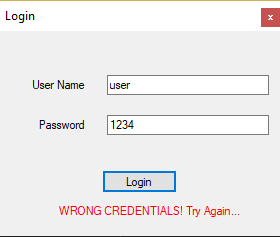
\includegraphics[scale=0.9]{images/tearordear/tear}
  \captionof{figure}{Login fallida en TearOrDear.exe}
  \label{fig:tear}
\end{figure}


Al abrir dnSpy, comenzamos revisando todos los archivos de TearOrDear, sin mucho exito en la mayoria, pues no hay información relevante, hasta que en la pestaña \texttt{button1\_Click} (\textbf{Ver Figura \ref{fig:button}}), nos encontramos con \textbf{if(this.username == this.o \&\& this.check1(s))}. Por cómo está escrito el código inferimos que es el chequeo que hace el programa para revisar si los parámetros del password son correctos o incorrectos \textbf{(Ver Figura \ref{fig:user})}

\begin{figure}[h]
  \centering
  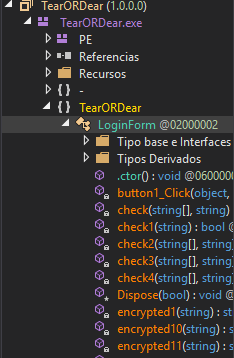
\includegraphics[scale=0.9]{images/tearordear/button}
  \captionof{figure}{Ubicación de texttt{button1\_Click}}
  \label{fig:button}
\end{figure} 

\begin{figure}[h]
  \centering
  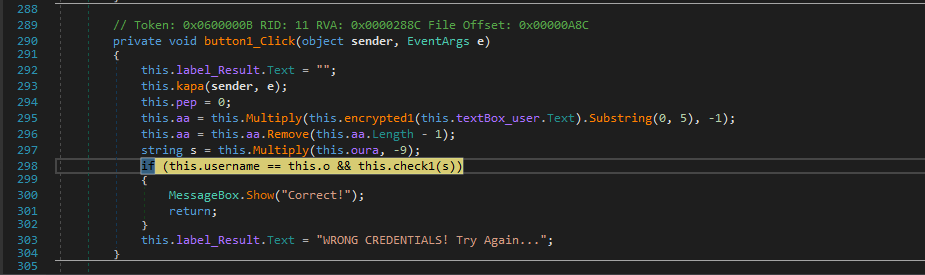
\includegraphics[scale=0.75]{images/tearordear/user}
  \captionof{figure}{Contenido función texttt{button1\_Click}}
  \label{fig:user}
\end{figure}
\newpage

Para que la condición sea verdadera, el \textit{username}, en mi caso 1234, debe tener el mismo valor que la variable \textbf{o} y además la función \textbf{check1} debe devolver verdadero.

Al buscar el valor de \textbf{o} observamos que vale \textbf{roiw}!$@$\# \textbf{(Ver Figura \ref{fig:user})}

\begin{figure}[h]
  \centering
  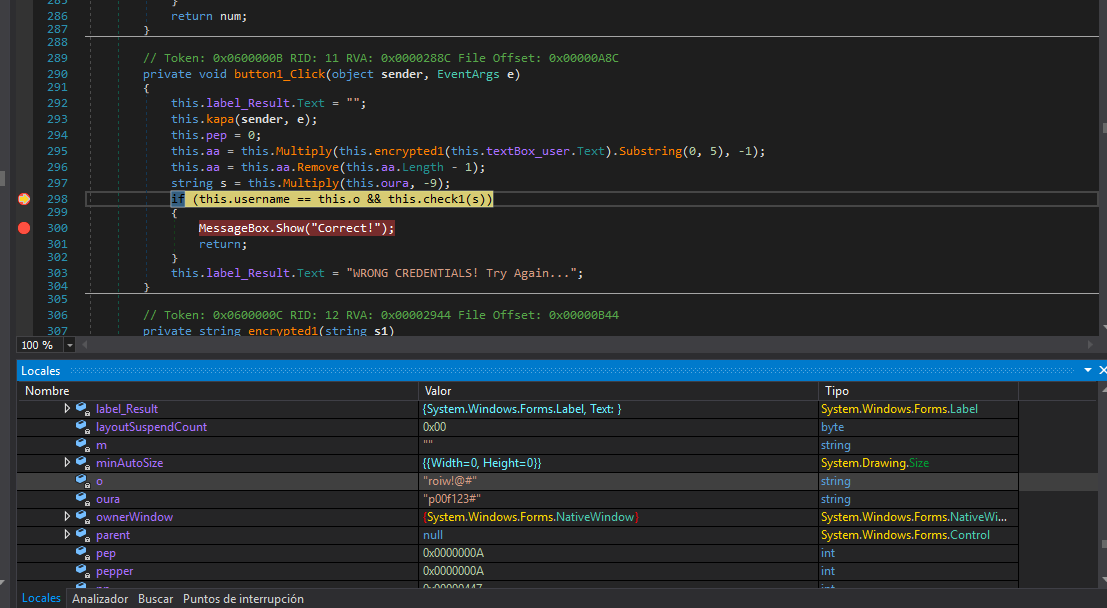
\includegraphics[scale=0.6]{images/tearordear/archivoo}
  \captionof{figure}{Resultado al generar una ruptura en la linea 298 del código, password}
  \label{fig:archivoo}
\end{figure} 

\newpage

Luego de realizar lo anterior, revisamos la función \textbf{check} que devuelve verdadero si lo que hemos introducido en \textbf{textBox\_user}, en nuestro caso \textit{user} es igual a la variable \textbf{aa} y también si el \textbf{array[0]} es igual a \textbf{array[22]} que siempre es verdad pues ambos son ``q''.

\begin{figure}[h]
  \centering
  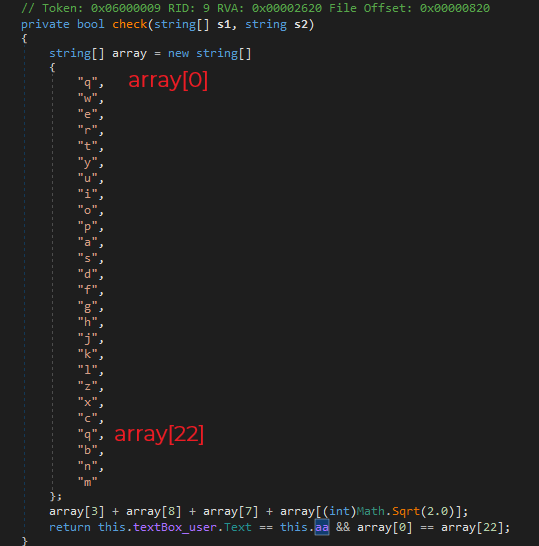
\includegraphics[scale=0.8]{images/tearordear/check}
  \captionof{figure}{Función check con return}
  \label{fig:check}
\end{figure} 

\newpage

Al revisar el valor de \textbf{aa} (Ver Figura \ref{fig:user_p}) vemos que el usuario debería ser igual a \texttt{piph}

\begin{figure}[h]
  \centering
  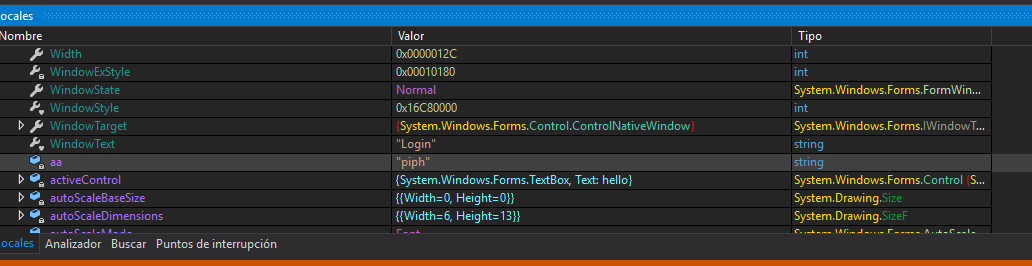
\includegraphics[scale=0.65]{images/tearordear/user_p}
  \captionof{figure}{Resultado al generar una ruptura en la linea 298 del código, user}
  \label{fig:user_p}
\end{figure} 

Comprobamos que estamos en lo cierto (Ver Figura \ref{fig:correct})

\begin{figure}[h]
  \centering
  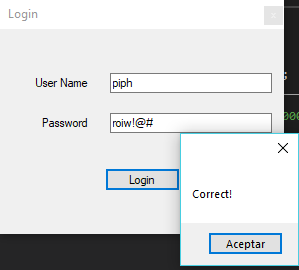
\includegraphics[scale=0.9]{images/tearordear/correct}
  \captionof{figure}{User y Password correctos}
  \label{fig:correct}
\end{figure} 

\newpage

Como el flag es HTB{username:password}, obtenemos el resultado.

\textbf{Flag: }HTB\{piph:roiw!$@$\#\}

\end{document}
